%%%%%%%%%%%%%%%%%%%%%%%%%%%%%% -*- Mode: Latex -*- %%%%%%%%%%%%%%%%%%%%%%%%%%%%
%% 04-14.tex -- IEEE Software Paper on Telemetry
%% Author          : Philip Johnson
%% Created On      : Mon Sep 23 11:52:28 2004
%% Last Modified By: Aaron Kagawa
%% Last Modified On: Sat Oct  9 15:28:54 2004
%% RCS: $Id$
%%%%%%%%%%%%%%%%%%%%%%%%%%%%%%%%%%%%%%%%%%%%%%%%%%%%%%%%%%%%%%%%%%%%%%%%%%%%%%
%%   Copyright (C) 2002 Philip Johnson
%%%%%%%%%%%%%%%%%%%%%%%%%%%%%%%%%%%%%%%%%%%%%%%%%%%%%%%%%%%%%%%%%%%%%%%%%%%%%%%
%% 

\documentclass[11pt,twocolumn]{article} 
\input{/export/home/csdl/tex/psfig/psfig}
\usepackage{/export/home/csdl/tex/icse2003/latex8}
\usepackage{times}
%% A verbatim-like environment which allows font changes
%%\usepackage{alltt}
%% New LaTeX2e graphics support
\usepackage[final]{graphicx}
% uncomment the % away on next line to produce the final camera-ready version
% and uncomment the \thispagestyle{empty} following \maketitle
\pagestyle{empty}

\begin{document}

\title{Optimizing the Initiation Phase of Software Inspections}

\author{\protect\begin{tabular}{ccc}
Aaron A. Kagawa \\
\end{tabular}\\
\em  Collaborative Software Development Laboratory \\
\em  Department of Information and Computer Sciences \\
\em  University of Hawai'i \\
\em  Honolulu, HI 96822 \\
\em  kagawaa@hawaii.edu}
\maketitle
\thispagestyle{empty}

\begin{abstract}  % 200 words
It is widely accepted that conducting Software Inspections results in high
software quality. However, in order to get the best results, the
Inspection process must be followed perfectly. Furthermore, many
organizations simply do not have the resources to conduct inspections on
every line of code due to time and cost constraints.

One of the major flaws in Software Inspection is the Initiation Phase. In
this phase, authors volunteer documents as canidates for inspection.  This
process of initiating an Inspection does not consider whether the document
will provide an adequate Return On Investment.

This research investigates whether it is possible for quality measures to
distinguish documents that are in ``most need of review'' from those in
``least need of review''. In some sense it flips the ``process of
Inspection leads to an increase of quality'' to ``an understanding of
quality will make Inspection more productive''. It is my claim that this
determination will help create an optimum Inspection Initiation Phase where
the ROI is high.
\end{abstract}

\Section{Introduction}
\label{sec:intro}
The use of Software Inspections has reported outstanding results in
improved productivity and quality. In fact, one study has found that if the
Inspection process is followed perfectly, then up to 95 percent of defects
can be removed before entering the testing phase \cite{Bush90}.
Inspections have been so successful that is likely to be the closest thing
we have to a ``silver bullet'' for improving software quality.  If this is
the case, then why is it that only small fraction of all software projects
conduct Inspections?  A study in the 1989 IEEE Transactions of Software
Engineering found that 84 percent of organizations participating in the
study performed some type of inspection process, but none performed
Inspections perfectly \cite{Bisant89}.

It is obvious that for some reason Software Inspection is hard to do
perfectly. Perhaps, the education of Software Inspection is too costly,
time constraints do not permit the many meetings needed to devote to
Inspections, or even the size of code affects whether Inspections can be
conducted on a large percentage of a project. For whatever reason,
project managers are either choosing not to conduct Inspections or doing
Inspections half-heartedly. In many cases, most development teams realize
that Inspections are useful, but cannot devote the resources necessary to
inspect all of the code.

The correct Software Inspection process begins with the Initiation Phase,
in which authors volunteer their documents for inspection.  The Inspection
Leader then checks the document against an entry criteria to determine if
the document is worth inspecting \cite{Gilb93}. I believe that this phase
of Inspection is a major problem; the process does not consider that some
documents are ``better'' to review than others. A simple illustration of
this fact is that 80 percent of defects come from 20 percent of the modules
\cite{Boehm01}. Thus, volunteering a document from that 20 percent will
likely be ``better'' than in any other module.

The goal of this research is to optimize the selection of documents for
review in the Initiation Phase. To do this I will create a Hackystat
extension that will determine what packages are in ``most need of review''
versus packages that are in ``least need of review''.

There are several research questions that I must answer in order to
successfully optimize the Initiation Phase of Inspections. The most
important question is the operational definition of the general terms
``most need'' and ``least need''. What software attributes can quanifiably
distinguish between ``most'' and ``least'' need of review. In order to
create a definition we must understand the motivation for Inspections.

Software Inspection has two primary goals; increase quality and
productivity. For this research I am primarily concerned with increasing
quality. The successful Inspection of a document has two main results:
finding defects which, once removed, increases software quality or not
finding defects thus indicating high software quality. Software quality is
vaguely defined as ``The degree to which software possess a desired
combination of attributes'' \cite{IEEEGlossary83}. Some of the possible
attributes can include; portability, reliability, efficiency, usability,
testability, understandability, and modifiability \cite{Glass03}. Some
other widely accepted measures of quality include defect density and
complexity.  Whatever definition used for quality, Inspections aim to
increase or validate the level of quality in software. Therefore, I would
claim that the same attributes defining software quality also provide good
indications of what code to inspect. For example, finding code that has low
portability, reliability, efficiency, usability, testability,
understandability, and modifiability would be a good indication of code
that would be beneficial to inspect.

My thesis claim is as follows: 
\begin{enumerate}
\item The attributes that define software quality provide good indications
  of what code to inspect.
\item Code that represents ``high'' software quality will have a low number
  of defects found in inspection.
\item Code that represents ``low'' software quality will have a high number
  of defects found in inspection.
\end{enumerate}

\Section{Evaluation Methodology}
\label{sec:evaluation}
To evaluate my thesis claims, I will create a Hackystat Extension that will
determine what packages are in ``most need of review'' from `packages that
are in ``least need of review''. When the system makes a determination of
what packages will provide the best ROI, I will recommend a package for
review. The results of the review (i.e. number of critical issues) will
determine if the package accurately reflected the ``most'' and ``least''
need of review determination.  To do this, I first need to gain a basic
understand of the attributes that affect quality.

It is important to note that I am not defining a set of attributes that
represent quality for all software projects. Instead, by using the
Hackystat Extension I will be able to go through a methodology to best
calibrate the attributes to accurately reflect the quality for the project
that I am studying.

For this evaluation, I will study the implementation of the Hackystat
System developed in the Collaborative Software Development Laboratory, of
the University of Hawaii at Manoa. Although, this is a project to which I
also contribute, I will minimize any possible data contamination by doing
two things. First, I will keep the results of the ``most'' and ``least''
need of review a secret both during and after conducting reviews. Second, I
will not participate in the reviews themselves.

To evaluate claim 1, I will conduct several weekly mini-studies to
fine-tune my calculation of quality. I will begin my study with several
basic attributes defined in the literature that are believed to affect
quality. Some of these attributes include size and coverage. Based on the
quality level, I will then recommend a specific package for review by the
CSDL staff. After the review, I will analyze the number of valid issues
generated and their severity. Thus, I will be able to conclude if the
quality level actually reflected a package that was in most need of review.
I will continue to fine-tune the attributes of quality on a weekly basis.
Once I have verified the attributes of quality, I can begin to evaluate
claim 2 and 3.

To evaluate claim 2 and 3, I will leave the attributes constant over a 6
week period and review three high quality and three low quality packages.
If my selected attributes are correct then the high quality packages should
have considerably less issues generated by review than the low quality
packages.

\Section{Hackystat Quality Extension}
This section provides a short description of the Hackystat Quality
Extension system. This system extends the functionality of the Hackystat
System to provide the ``most'' and ``least'' need of review determinations.

The Hackystat System provides several Sensor Data Types which represent
quantitative data about both the product and development process of a
software project. Using this data I will build attributes that represent
quality. For example, some of the attributes that are currently possible
are the following:

\begin{enumerate}
\item Active Time
\item Number of Changes (Commits)
\item Date of Last Change
\item Number of Inspections
\item Date of Last Inspection
\item Number of Defects
\item Date of Last Defect
\item Lines of Code, Number of Methods, and Number of Classes
\item Lines of Test Code, Number of Test Methods, and Number of Test
Classes
\item Coverage
\end{enumerate}

Currently, each of these attributes is collected for each package or
workspace within a specified project. Figure 1 shows several example high
quality (or ``least need of review'') workspaces with their respective
attributes of quality.

\begin{figure*}[ht]
  \centering
  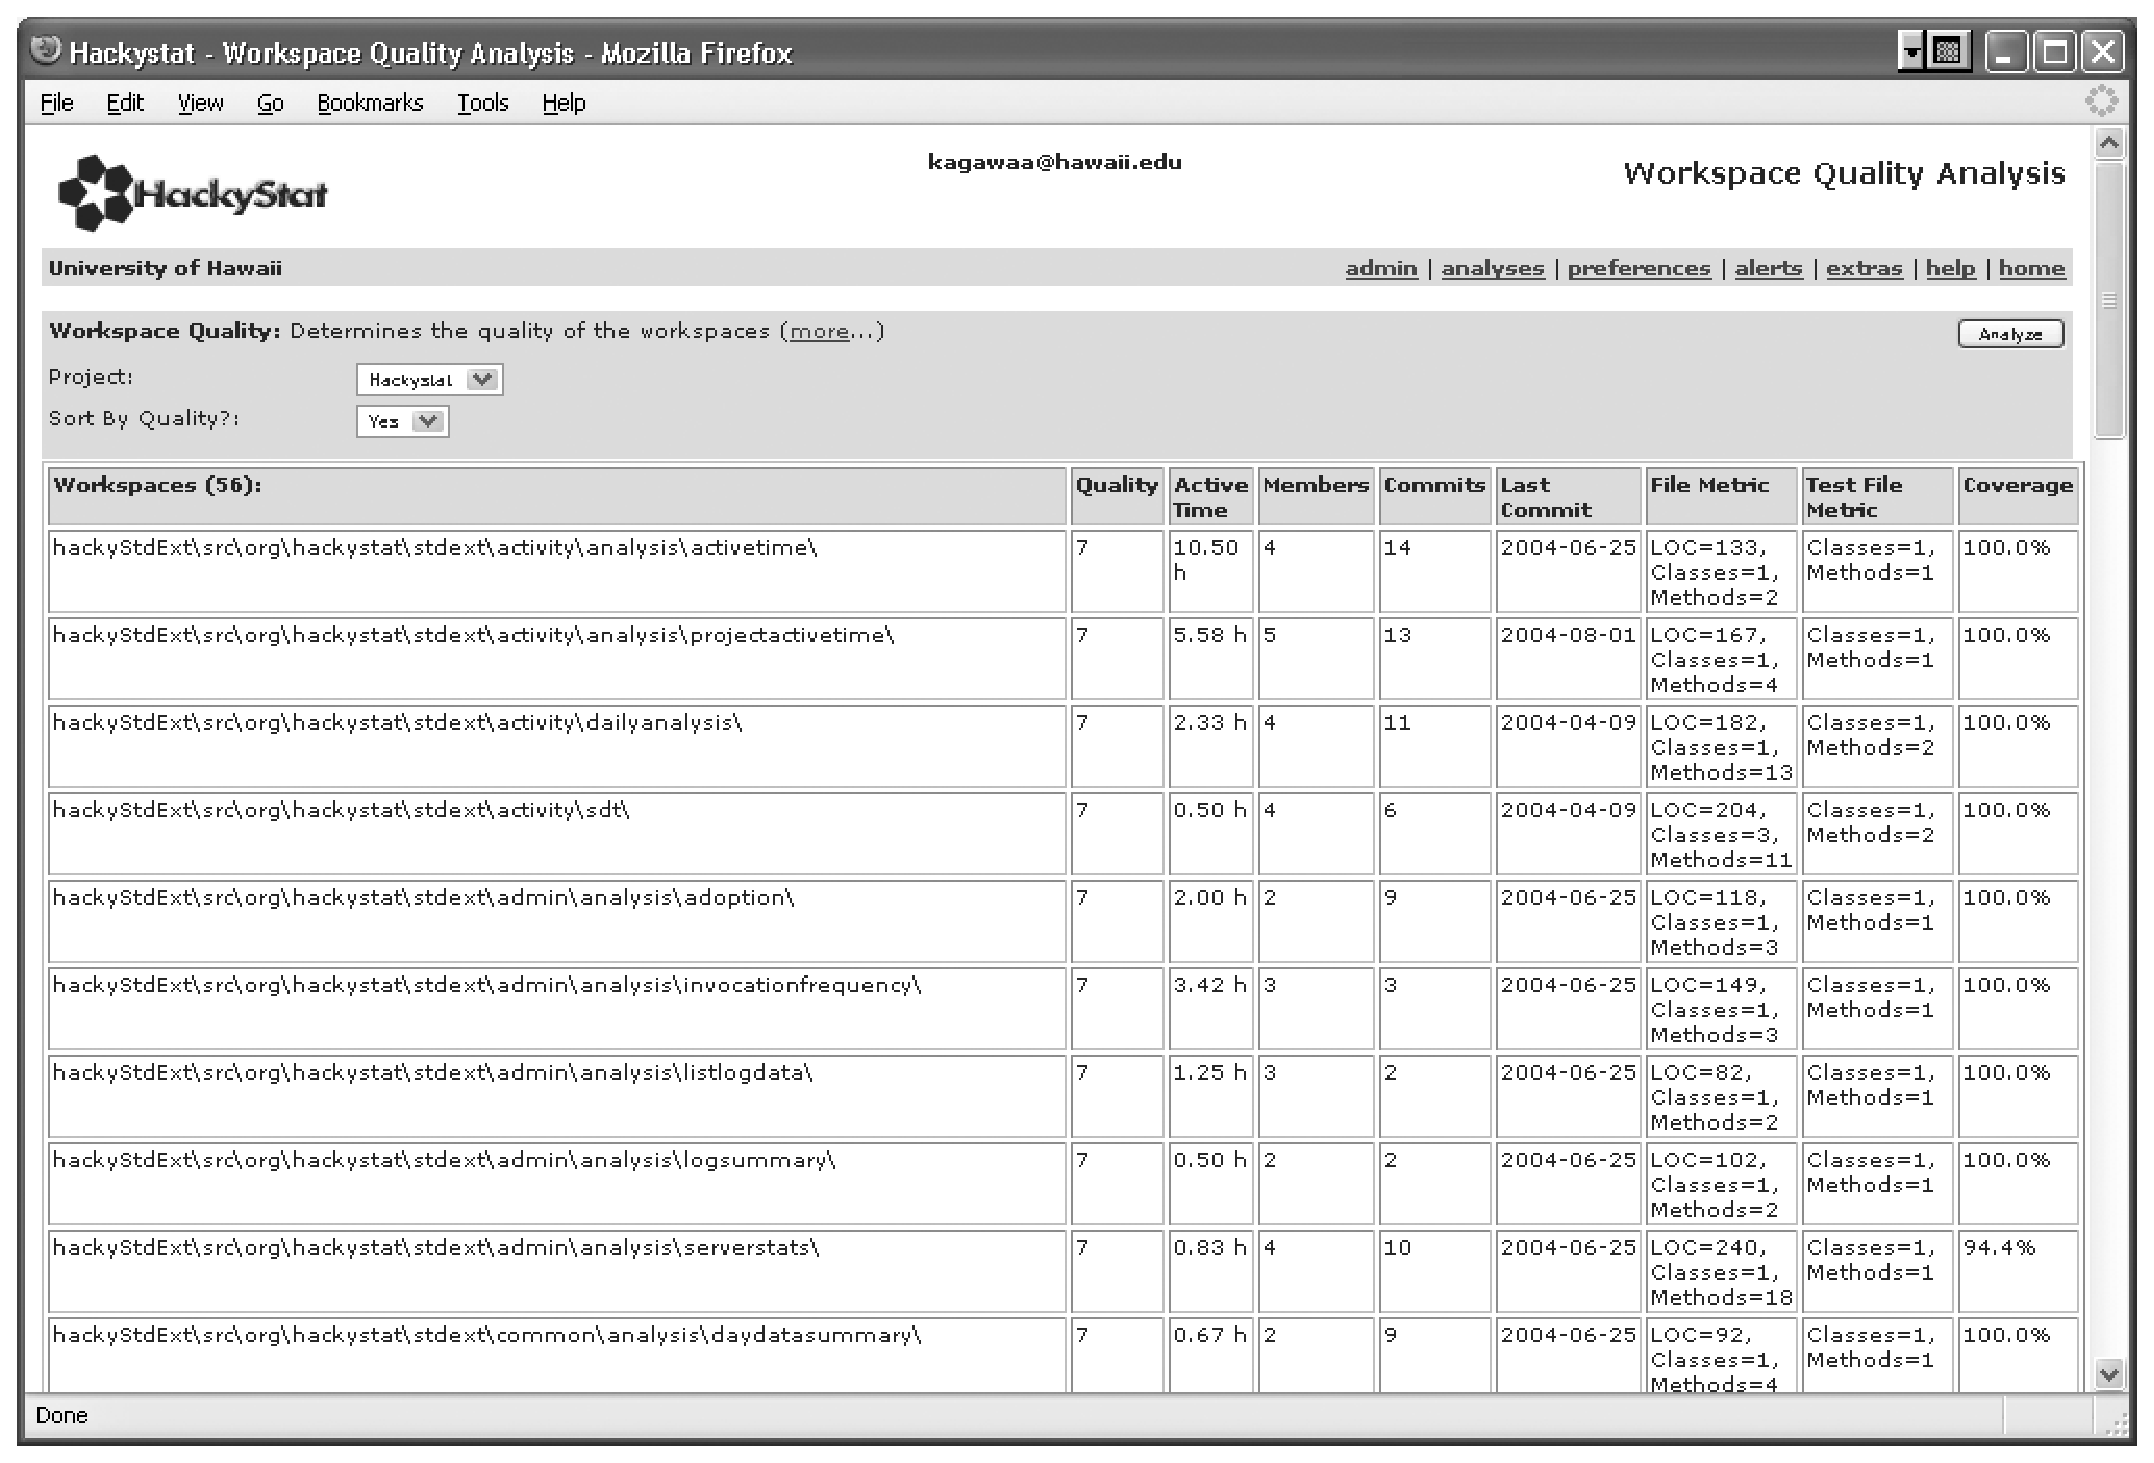
\includegraphics[width=1.00\textwidth]{WorkspaceQuality.eps}
  \caption{The Workspace Quality analysis. Workspaces are listed with its
  respective quality level and the attributes that make up its quality
  level.
}
  \label{fig:WorkspaceQualityAnalysis}
\end{figure*}

To make the important determination of ``most'' and ``least'' need of
review, I assign certain quality levels or numerical weights to the
attributes. For example, if the coverage of a package is below 80 percent,
I assign a ``low'' quality level for that attribute. Likewise, if the
coverage of a package is a 100 percent, then I assign a ``high'' quality
level. ``Low'' is operationalized by a 1, ``high'' is operationalized by a
3, and ``middle ground'' is operationalized by a 2. The system assigns each
attribute a quality level, then assigns each package an aggregated quality
level which is the sum of the quality levels associated with its
attributes. The packages are then sorted by the packages' aggregate quality
level, sorting the ``most need of review'' to the bottom and ``least need
of review'' to the top.

There are several issues with the assignment of numerical weights (or
quality levels as I call them) that I still need to address. For example, I
explicitly determine the quality levels using my own subjective measure of
what is low versus high quality. I will need to explore if my subjective
measure is sufficient, if some attributes should be weighted more than
others, or if any other entirely different weighting methods provide more
accurate results.

\Section{Initial Results}
The use of the Hackystat Quality Extension system to provide the
determination of ``most'' and ``least'' need of review has been promising.
The initial implementation of the system has proven that it is technically
possible to do what I have envisioned. In addition, I have already
recommended the review of a package that was in ``most need of a review''
and the defects and issues identified has confirmed that the package had
low quality.

Of course, I will continue to discover new attributes to define quality,
fine tune the numerical weights associated with the attributes, and
continue to recommend reviews until I believe my mechanism is ready for a
thorough evaluation.

\Section{Contributions}
If I find evidence that my thesis claims are true, then I believe the
formal Software Inspection process should address some sort of quantitative
approach for initiating inspections. An optimized Initiation Phase will
narrow down the number of possible documents to inspect and it will also
provide the best Return On Investment possible. 

In addition, I believe that the system's quantification of quality is
valuable in of itself. Development teams can use the system's attributes of
quality to guide the management of quality.

\bibliographystyle{/export/home/csdl/tex/icse2003/latex8}
\bibliography{/export/home/csdl/techreports/04-14/04-14,/export/home/csdl/bib/csdl-trs,/export/home/csdl/bib/hackystat,/export/home/csdl/bib/ftr}
\end{document}




